\section*{Working Principle of the Experiment}
working principle of the experiment will go here......
\begin{figure}[h]
\begin{center}
 
\includegraphics[width=.4\linewidth]{demo_image1} % You can add theoritical graphs
  \caption{Title of the image}\label{Fig:Figure1}
\end{center}
\end{figure}




\section*{Equipment }
\begin{enumerate}
    \item Item 1
    \item Item 2
    \item Item 3
    \item Item 4
    \item Item 5
\end{enumerate}

\section*{Experimental Data  }
Text on experimental data and table go here.........
\begin{figure}[h]
\begin{center}
 
\includegraphics[width=.4\linewidth]{demo_image1} % You can add Experimental data                                                   picture here.......
 \caption{Title of the image}\label{Fig:Figure2}
\end{center}
\end{figure}


\section*{Experimental Graph}

\begin{figure}[h]
\begin{center}
 
\includegraphics[width=.4\linewidth]{demo_image1} % You can add Experimental graph                                                   picture here.......
 \caption{Title of the image}\label{Fig:Figure3}
\end{center}
\end{figure}
\newpage
\section*{Error Calculation }
Write the error analysis in this section.................
\begin{figure}[ht]
   \begin{minipage}{0.48\textwidth}
     \centering
     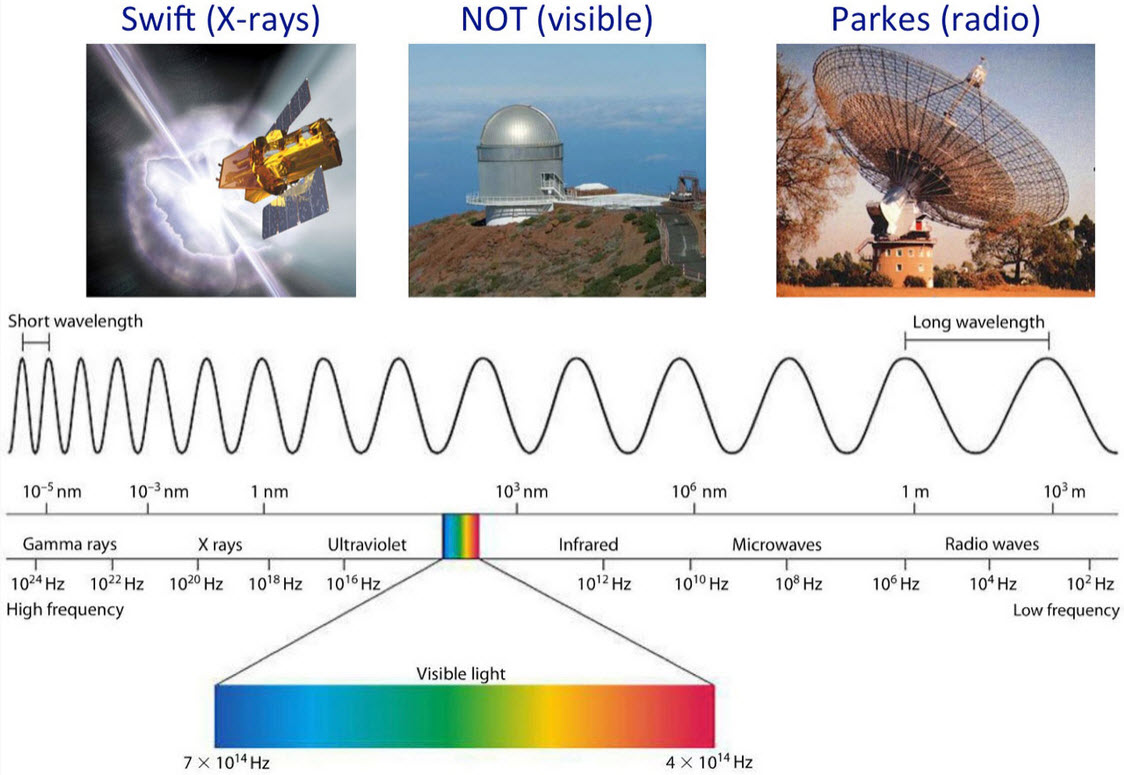
\includegraphics[width=.8\linewidth]{demo_image2}
     \caption{Ideal Graph}\label{Fig:Data1}
   \end{minipage}\hfill
   \begin{minipage}{0.48\textwidth}
     \centering
     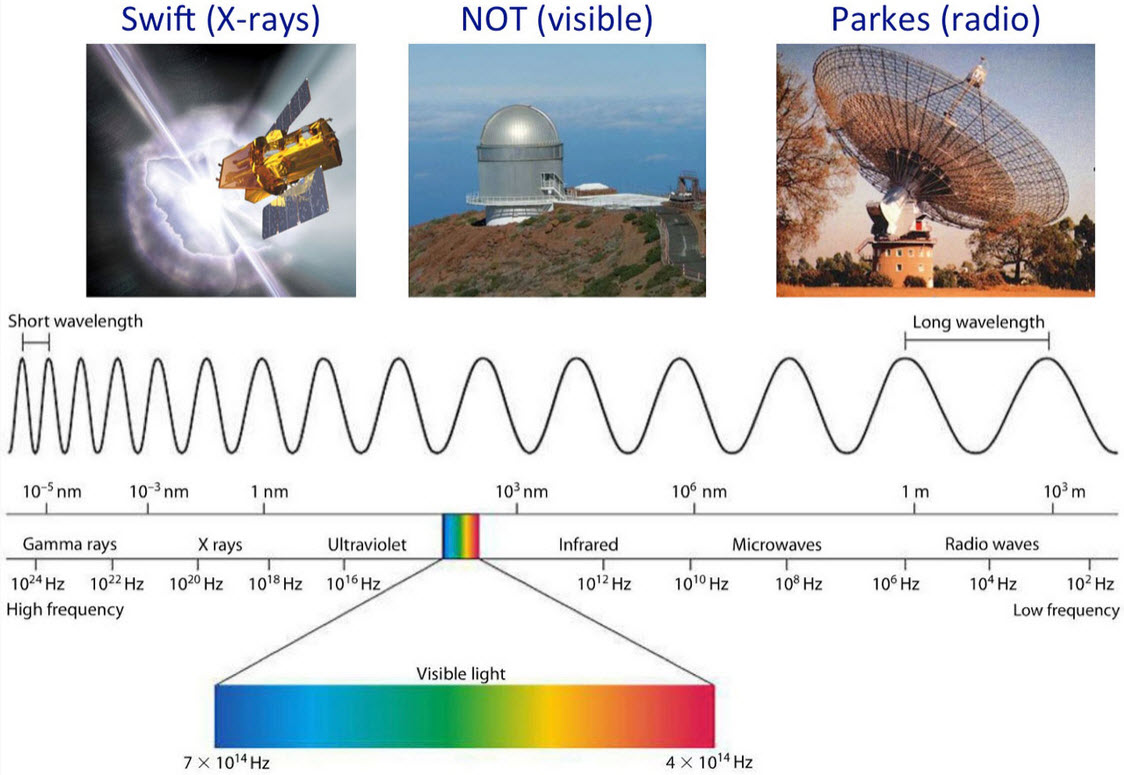
\includegraphics[width=.8\linewidth]{demo_image2}
     \caption{Actual Graph}\label{Fig:Data2}
   \end{minipage}
\end{figure}